\section{Applications}
\label{sec:applications}

In this final section of \myref{chapter}{chap:linear-systems}, we focus on some
`real-world' applications of linear systems and, more generally, on methods of
solving linear systems using computers.

The software we shall employ toward this end styles
\href{https://www.sagemath.org/}{SageMath}. It's a free open-source mathematics
software capable of numeric and symbolic manipulation of objects from various
fields of mathematics, linear algebra included. It can be installed on most
operating systems following the
\href{https://doc.sagemath.org/html/en/installation/index.html}{official guide}.

SageMath is essentially a terminal-based software and out of the box offers no
graphical user interface. Upon launch, the user is greeted by a screen similar
to this one:
\begin{Verbatim}
┌────────────────────────────────────────────────────────────────────┐
│ SageMath version 10.4, Release Date: 2024-07-19                    │
│ Using Python 3.12.8. Type "help()" for help.                       │
└────────────────────────────────────────────────────────────────────┘
sage:
\end{Verbatim}
SageMath is mainly built upon C and Python and is \emph{interpreted}, meaning
every piece of code is immediately run without a need for compilation.

Before we focus on applications of linear systems in fields like
\emph{economics} and \emph{physics}, we need to learn to solve them using
SageMath. By far the simplest way to encode linear systems is using matrix
notation. SageMath features the \texttt{Matrix} class which hosts a plethora of
methods for matrix manipulation we are going to make great use of in time.

\myref{Example}{exam:static-equations} contains the system
\[
 \left(
  \begin{matrix*}[r]
   15 & 40\\
   25 & -50
  \end{matrix*}
  \hspace{1mm}
 \right|
 \left.
  \begin{matrix*}[r]
   100\\
   50
  \end{matrix*}
 \right).
\]
Let us solve it using SageMath. The \texttt{Matrix} class expects a matrix to be
defined as a list of rows which are themselves lists of elements. In addition,
we may specify the number set wherein the elements lie. For example,
\begin{Verbatim}
sage: A = \clb{Matrix(}ZZ, [
....:     [\clr{15}, \clr{40}],
....:     [\clr{25}, \clr{-50}],
....: ]\clb{)}
\end{Verbatim}
creates the matrix
\[
 \left(
  \begin{matrix*}[r]
   15 & 40\\
   25 & -50
  \end{matrix*}
 \right)
\]
with entries in $\Z$, the integers. This has a caveat. When we tell SageMath our
matrix contains entries \emph{exclusively} in $\Z$, it will fulfil our wish with
utmost conscientiousness. This means that \texttt{A} can never contain anything
but integers. A problem might emerge should we wish to put it into echelon form
for example. Gauss-Jordan elimination of the matrix \texttt{A} would clearly
require subtracting $(25 / 15)$-multiple of row \texttt{I} from row \texttt{II}.
Assuming the entries of \texttt{A} are solely integers, such an operation is not
permitted. The \texttt{Matrix} class has an in-built method for Gauss-Jordan
elimination. Let us try to use it.
\begin{Verbatim}
sage: A.\clb{echelon_form()}
[  \clr{5} \clr{130}]
[  \clr{0} \clr{350}]
\end{Verbatim}
The result is somewhat unexpected. Thankfully or unfortunately, SageMath is
clever enough to know that simply following the algorithm of the Gauss-Jordan
elimination does not yield an integer matrix. So, it instead follows the
algorithm and then multiplies the matrix by the least common multiple of the
denominators of all entries in order to yield an integer matrix. Beware however,
that trying to solve linear systems whose solutions are rational with integer
matrices might result in an error. To stay in the clear, we instead use the real
numbers throughout the calculation. Not specifying the number set would lead to
SageMath `guessing' it based on the values of the entries -- which are all
integral.

We thus rewrite our matrix \texttt{A} like this:
\begin{Verbatim}
sage: A = Matrix(\clb{RR}, [
....:     [\clr{15}, \clr{40}],
....:     [\clr{25}, \clr{-50}],
....: ])
\end{Verbatim}
We will also create a \texttt{vector} (a \texttt{Matrix} with a single row
basically) of the right hand side of the studied system.
\begin{Verbatim}
sage: b = \clb{vector(}RR, [\clr{100}, \clr{50}]\clb{)}
\end{Verbatim}
The \texttt{Matrix} method for solving a system with a given \texttt{vector} of
right hand side is called \texttt{solve\_right}. Using it gives
\begin{Verbatim}
sage: A.\clb{solve_right(}b\clb{)}
(\clr{4.00000000000000}, \clr{1.00000000000000})
\end{Verbatim}
Since we explicitly required SageMath solve the system over the real numbers, it
returned the solution as a pair of decimals rounded based on a default precision
parameter. We would instead prefer to write the solution as $(4,1)$. Should we
wish to record the solution as a pair of fractions or integers instead, we would
need to define \texttt{A} and \texttt{b} over $\Q$.
\begin{Verbatim}
sage: A = Matrix(\clb{QQ}, [
....:     [\clr{15}, \clr{40}],
....:     [\clr{25}, \clr{-50}],
....: ])
sage: b = vector(\clb{QQ}, [\clr{100}, \clr{50}])
sage: A.solve_right(b)
(\clr{4}, \clr{1})
\end{Verbatim}

\subsection{Numerical Stability}
\label{ssec:numerical-stability}

Numerical stability (of a linear system) refers to one of its computational
qualities -- the quality described often as `small change in input causes a
small change in output'. As real numbers are represented in computer memory with
a given precision (more or less the number of decimal places), deviations in
input data small enough to go unnoticed may cause issues. We shall highlight two
of said `issues' (and possible countermeasures) in this subsection.

Consider the system
\begin{equation}
 \label{eq:same-eq-twice}
 \begin{array}{r c r c r}
  2x & + & y & = & 3\\
  2x & + & y & = & 3
 \end{array}
\end{equation}
with infinitely many solutions of the form $((3-y) / 2, y)$. Now, altering the
system slightly
\[
 \begin{array}{r c r c r}
  2x & + & y & = & 3\\
  2.000000002x & + & 1.000000001y & = & 3.000000003
 \end{array}
\]
yields a system with exactly one solution -- $(1,1)$. We see that immediately
but a computer with limited precision might regard this altered system exactly
the same way as the previous one. Should we draw the system, we would basically
see just one line given that the size of the angle between the lines
corresponding to the two equations is negligible.

Systems where two or more equations are indistinguishable with low enough
precision are typically called \emph{ill-conditioned}. In this case, there is
not much that can be done to alleviate the problem. See for yourself.
\begin{Verbatim}
sage: A = Matrix(RR, [
....:     [\clr{2}, \clr{1}],
....:     [\clr{2} + \clb{2*10**-18}, \clr{1} + \clb{10**-18}],
....: ])
sage: b = vector(RR, [\clr{3}, \clr{3} + \clb{3*10**-18}])
sage: A.solve_right(b)
(\clr{1.50000000000000}, \clr{0.000000000000000})
\end{Verbatim}
The solution given by SageMath is clearly wrong because of the \clb{tiny
deviation} in input data. It instead computed the solution to the
system~\eqref{eq:same-eq-twice} and substituted $y = 0$, which is default
behaviour.

Next, we take a look at the system
\[
 \begin{array}{r c r c r}
  \frac{1}{1000}x & + & y & = & 1\\
  x & - & y & = & 0
 \end{array}
\]
with unique solution $(1000 / 1001, 1000 / 1001)$. Here, depending on the order
of the equations, computers can arrive at a wrong solution. In the first step of
Gauss-Jordan elimination, we subtract a $1000$-multiple of row \texttt{I} from
row \texttt{II}, obtaining
\begin{equation}
 \label{eq:wrong-order}
 \begin{array}{r c r c r}
  \frac{1}{1000}x & + & y & = & 1\\
  & & -1001 y & = & -1000.
 \end{array}
\end{equation}
Even if we are working with enough precision to represent thousandths of
integers, the result of the computation
\[
 y = \frac{-1000}{-1001}
\]
may easily be rounded to $1$ due to the way computers perform division. As three
decimal places are hardly enough to push modern computers to their limits, see
the following example instead.
\begin{Verbatim}
sage: a = \clr{-1 * 10**18}
sage: b = \clr{-1 * 10**18 - 1}
sage: \clb{numerical_approx}(a / b)
\clr{1.00000000000000}
\end{Verbatim}
The \texttt{numerical\_approx} function tells SageMath to represent $a / b$ as a
real number, otherwise it would have stored it as a fraction.

Should we now begin the process of back-substitution in the
system~\eqref{eq:wrong-order}, we would inevitably get a wrong solution. If the
second equation yields (with low precision) that $y = 1$, then from the first
equation, we get $x = 0$. This is a \emph{completely} different solution from
the exact one. The difference between $(0,1)$ and $(1000 / 1001, 1000 / 1001)$
might not seem too high but imagine $x$ and $y$ represented \emph{percentages}
for example. Then, instead of both $x$ and $y$ being nearly $100\%$, $x$ gets
smashed down all the way to $0 \%$.

Perhaps a little surprisingly, this problem can be \emph{thoroughly} solved by
simply changing the order of the equations. If we had instead used Gauss-Jordan
elimination to solve the system
\[
 \begin{array}{r c r c r}
  x & - & y & = & 0\\
  \frac{1}{1000}x & + & y & = & 1,
 \end{array}
\]
we wouldn't have run into any issues. Indeed, the first step here entails
subtracting $(1 / 1000)$-multiple of row \texttt{I} from row \texttt{II}. This
yields
\[
 \begin{array}{r c r c r}
  x & - & y & = & 0\\
  & & \frac{1001}{1000}y & = & 1.
 \end{array}
\]
This time, even if $1001 / 1000$ \emph{does} get rounded to one, the exact
solution will still be reached with sufficient degree of accuracy. Supposing the
second equation is evaluated to be true if $y = 1$, the first equation then
gives $x = 1$. Clearly, the number $1000 / 1001$ is much closer to $1$ than it
is to $0$.

All in all, there exist cases where additional steps performed during
Gauss-Jordan elimination greatly increase the accuracy of the approximation of
potential solutions of a linear system. One very simple and statistically
effective method is to always swap the row which is to be used for elimination
of other rows with the row with highest (in absolute value) pivot coefficient.
The reason this works is that computers are, vaguely speaking, prone to rounding
numbers that \emph{are not} close to $0$. This method is exactly what we
employed here, by the way. Instead of solving
\[
 \begin{array}{r c r c r}
  \frac{1}{1000}x & + & y & = & 1\\
  x & - & y & = & 0
 \end{array}
\]
we swapped row \texttt{I} with row \texttt{II} as row \texttt{II} has a
$1000$-times larger coefficient of the variable $x$ than row \texttt{II}. In the
next section, we intend to show how Gauss-Jordan elimination can be coded in
SageMath while also including the aforementioned `accuracy-improving' step.

\begin{exercise}{}{bad-accuracy-system}
 Devise a linear system the accuracy of the solution whereof suffers from
 insufficient precision but falls into neither of the two categories described.
\end{exercise}

\subsection{Gauss-Jordan Elimination Revisited}
\label{ssec:gauss-jordan-elimination-revisited}

Here, we provide a fully algorithmic description of the Gauss-Jordan elimination
algorithm discussed in \myref{section}{sec:gauss-jordan-elimination} and also
one possible way of encoding it in SageMath. Here goes nothing.
\begin{algorithm}[H]
 \SetAlgoVlined
 \SetKwInOut{Input}{input}
 \SetKwInOut{Output}{output}

 \Input{An $n \times m$ matrix $A = (a_{i,j})_{i=1,j=1}^{n,m}$ with real
 entries.}
 \Output{The matrix $A$ in echelon form.}
 \BlankLine
 \tcc{Row to be used for elimination of other rows.}
 $r \leftarrow 1$;\\

 \BlankLine
 \tcc{Traverse the columns.}
 \For {$c \in \{1,\ldots,m\}$}{
  \tcc{Find the row (below $r$) with maximal value in column $c$. Denote by $b$
  the row with the maximal currently known value.}
  $b \leftarrow r$;\\
  \tcc{Traverse the rows below $r$.}
  \For {$i \in \{r+1,\ldots,n\}$} {
   \If {$|a_{i,c}| > |a_{b,c}|$} {
    \tcc{Found a row with higher value in column $c$. Replace $b$ with $i$.}
    $b \leftarrow i$;
   }
  }
  \tcc{If $a_{b,c} = 0$, then move to next column since this column is full of
  zeroes.}
  \If {$a_{b,c} = 0$} {
   continue;
  }
  \BlankLine
  swap rows with indices $r$ and $b$;\\
  \tcc{Eliminate variables in column $c$ in all rows below $r$.}
  \For {$i \in \{r+1,\ldots,n\}$} {
   \For {$j \in \{c,\ldots,m\}$} {
    $a_{i,j} \leftarrow a_{i,j} - \frac{a_{i,c}}{a_{r,c}} a_{r,j}$;
   }
  }
  \BlankLine
  \tcc{Row $r$ now contains the pivot in column $c$ so it will remain the same
  for the rest of the algorithm. Move to the next row.}
  $r \leftarrow r + 1$;
 }
 \BlankLine
 \Return{$A$};
 \caption{Gauss-Jordan Elimination.}
 \label{algo:gauss-jordan-elimination}
\end{algorithm}

\begin{example}{}{gauss-jordan-elimination}
 Let's put the matrix
 \[
  A = \left( 
   \begin{matrix*}[r]
    2 & 0 & 1\\
    -1 & 1 & 1\\
    4 & 2 & 2
   \end{matrix*}
  \right)
 \]
 into echelon form using \myref{algorithm}{algo:gauss-jordan-elimination}. At
 first, we have $r = 1$ and $c = 1$. Going through rows $2$ and $3$, we see that
 the number with the highest value in column $1$ lies in row $3$. Hence, we
 first swap row $1$ with row $3$.
 \[
  A = \left( 
   \begin{matrix*}[r]
    4 & 2 & 2\\
    -1 & 1 & 1\\
    2 & 0 & 1
   \end{matrix*}
  \right)
 \]
 Now begins the process of elimination. Since $r = 1$, the index $i$ exhausts
 the set $\{2,3\}$. For $i = 2$, we calculate $a_{i,c} / a_{r,c}$ = $a_{2,1} /
 a_{1,1} = -1 / 4$. We thus subtract $(-1 / 4)$-multiple of row $1$ from row
 $2$. 
 \[
  A = \left( 
   \begin{matrix*}[r]
    4 & 2 & 2\\
    0 & \frac{3}{2} & \frac{3}{2}\\
    2 & 0 & 1
   \end{matrix*}
  \right)
 \]
 Next, we set $i \coloneqq 3$ and calculate $a_{i,c} / a_{r,c} = 1 / 2$; we then
 subtract $(1 / 2)$-multiple of row $1$ from row $3$.
 \[
  A = \left( 
   \begin{matrix*}[r]
    4 & 2 & 2\\
    0 & \frac{3}{2} & \frac{3}{2}\\
    0 & -1 & 0
   \end{matrix*}
  \right)
 \]
 Since all rows in column $c$ below $r$ have been eliminated, we move to the
 next row by setting $r \coloneqq 2$. We also move to the next column via $c
 \coloneqq 2$.

 Now, the number with the largest absolute value in column $c$ and all rows
 below (and including) $r$ already lies in row $r$, so no swap is needed. We
 perform the elimination of row $3$ by calculating $a_{3,c} / a_{r,c} = a_{3,2}
 / a_{2,2} = - 2 / 3$ and subtracting the $(-2 / 3)$-multiple of row $2$ from
 row $3$.
 \[
  A = \left( 
   \begin{matrix*}[r]
    4 & 2 & 2\\
    0 & \frac{3}{2} & \frac{3}{2}\\
    0 & 0 & 1
   \end{matrix*}
  \right)
 \]
 We move to the next row via $r \coloneqq 3$ and the next column via $c
 \coloneqq 3$. No further elimination takes place because there are no rows
 below row $3$. The matrix $A$ has been put into echelon form.
\end{example}

Before finally marching on, we present a way of implementing
\myref{algorithm}{algo:gauss-jordan-elimination} in SageMath. This
implementation almost aligns with the implementation of the algorithm in Python.
Let us be responsible adults and break it into functions.

The function for finding the row with the highest pivot coefficient in the
current row might look like this:
\begin{Verbatim}
sage: \clg{def} \clr{find_best_row}(A: \clb{Matrix}, cur_row: \clb{int}, cur_col: \clb{int}):
....:     best_row = cur_row
....:
....:     \clg{for} row_below \clg{in} \clr{range}(cur_row + 1, \clr{len}(A.\clr{rows}())):
....:         if \clr{abs}(A[row_below][cur_col]) > \clr{abs}(A[best_row][cur_col]):
....:             best_row = row_below
....:
....:     \clg{return} best_row
\end{Verbatim}
We also implement the function to eliminate the first non-zero element in all
rows below a given row.
\begin{Verbatim}
sage: \clg{def} \clr{eliminate_rows}(A: \clb{Matrix}, cur_row: \clb{int}, cur_col: \clb{int}):
....:     \clg{for} row_below \clg{in} \clr{range}(cur_row + 1, \clr{len}(A.\clr{rows}())):
....:         scalar = A[row_below][cur_col] / A[cur_row][cur_col]
....:         A[row_below] = A[row_below] - scalar * A[cur_row]
\end{Verbatim}
These are all the functions we need to cleanly implement Gauss-Jordan
elimination in SageMath.
\begin{Verbatim}
sage: \clg{def} \clr{eliminate}(A: \clb{Matrix}):
....:     cur_row = \clm{0}
....:
....:     \clg{for} cur_col \clg{in} \clr{range}(\clr{len}(A.\clr{columns}())):
....:         best_row = \clr{find_best_row}(A, cur_row, cur_col)
....:         A[cur_row], A[best_row] = A[best_row], A[cur_row]
....:
....:         \clg{if} A[cur_row][cur_col] == \clm{0}:
....:             \clg{continue}
....:
....:         \clr{eliminate_rows}(A, cur_row, cur_col)
....:         cur_row += \clm{1}
\end{Verbatim}
And, to wrap things up, a short application on the matrix from
\myref{example}{exam:gauss-jordan-elimination}.
\begin{Verbatim}
sage: A = \clb{Matrix}(QQ, [
....:     [\clr{2}, \clr{0}, \clr{1}],
....:     [\clr{-1}, \clr{1}, \clr{1}],
....:     [\clr{4}, \clr{2}, \clr{2}],
....: ])
sage: \clr{eliminate}(A)
sage: A
[  \clr{4}   \clr{2}   \clr{2}]
[  \clr{0} \clr{3/2} \clr{3/2}]
[  \clr{0}   \clr{0}   \clr{1}]
\end{Verbatim}

\subsection{Input-Output Analysis}
\label{ssec:input-output-analysis}

A place where linear systems naturally flourish is \emph{economics}. Put
briefly, economy is a network of mutually influenced industries. An important
observation is that this `influence' is mostly of \emph{linear} nature. We take
as an example the \emph{steel} and \emph{automobile} industries. Both of these
industries use its own output and the other industry's output to optimize
production. The steel industry might use steel to produce factories, and use
cars for the transport of goods between them. Similarly, the automobile industry
uses its own cars to transports its other cars and uses steel to produce them in
the first place. In economics, we're typically interested in predicting the
future value of an industry. However, in cases like these, it isn't intuitively
evident how the total value of steel used by external actors (meaning not the
steel or automobile industries) would influence the system, for example.

Suppose we accumulated the following data:
\begin{table}[ht]
 \centering
 \begin{tabular}{r | r | r | r | r}
  & \textbf{used by steel} & \textbf{used by auto} & \textbf{used by others} &
  \textbf{total}\\
  \toprule
  value of steel (in billions of \$) & 6.90 & 1.28 & 10.51 & 18.69 \\
  value of auto (in billions of \$) & 2.24 & 4.40 & 7.63 & 14.27
 \end{tabular}

 \caption{The annual summary of the value of steel and automobile industries.}
 \label{table:steel-and-automobile}
\end{table}

Based on this data, how ought we to attempt to predict the total values of steel
and automobile industries based on shifting external demand? First and foremost,
why do we care primarily about external demand? The answer is simple. As long as
external demand stays stable, it is improbable that the automobile industry
would suddenly produce more cars or that the steel industry more steel. It is
indeed mostly individual customers and other affiliated industries which cause a
change in production.

Suppose that the value of steel and automobile industries used externally in the
next year shifts by $d_s$ and $d_a$, respectively. How does this affect their
total value? To answer this, we need observe that the steel and automobile
industries form a linear system. Under the premise that the steel industry uses
the same \emph{fraction} of its own output and the automobile industry also uses
the same fraction of the steel industry output as this year, we can predict its
value next year (which we denote $s$) to equal
\[
 s = (6.90 / 18.69)s + (1.28 / 14.27)a + (10.51 + d_s).
\]
This formula essentially says the obvious:
\begin{align*}
 \text{next year's value of steel} &= \text{next year's value of steel used by
 steel}\\
                                   &+ \text{next year's value of steel used by
                                   auto}\\
                                   &+ \text{next year's value of steel used by
                                   others}.
\end{align*}
We are just predicting the next year values based on this year's ones while
keeping the ratios of output distribution stable.

Similarly, the equation for the predicted next year's total automobile industry
value (denoted $a$) is
\[
 a = (2.24 / 18.69)s + (4.40 / 14.27)a + (7.63 + d_a).
\]
Both of these linear equations put together form the linear system
\[
 \begin{array}{r c r c r c r}
  s & = & (6.90 / 18.69)s & + & (1.28 / 14.27)a & + & (10.51 + d_s)\\
  a & = & (2.24 / 18.69)s & + & (4.40 / 14.27)a & + & (7.63 + d_a)
 \end{array}
\]
An easy computation and rearrangement gives
\[
 \begin{array}{r c r c r}
  (11.79 / 18.69)s & - & (1.28 / 14.27)a & = & (10.51 + d_s)\\
  -(2.24 / 18.69)s & + & (9.87 / 14.27)a & = & (7.63 + d_a)
 \end{array}
\]
As we did many a time already, we collect the equations into a matrix $A$ and a
vector $b$ like so:
\[
 A = \left( 
  \begin{matrix*}[r]
   11.79 / 18.69 & -1.28 / 14.27\\
   -2.24 / 18.69 & 9.87 / 14.27
  \end{matrix*}
 \right), \quad \mathbf{b} = \left( 
  \begin{matrix*}[r]
   10.51 + d_s\\
   7.63 + d_a
  \end{matrix*}
 \right).
\]
Fortunately, SageMath has in-built support for variables. We can thus let it
solve the system for us and represent the solution in terms of variables $d_s$
and $d_a$.
\begin{Verbatim}
sage: \clr{var}(\clbr{'ds da'})
(\clbr{ds}, \clbr{da})
sage: A = \clb{Matrix}([
....:     [\clr{11.79/18.69}, \clr{-1.28/14.27}],
....:     [\clr{-2.24/18.69}, \clr{9.87/14.27}],
....: ])
sage: b = \clb{vector}([\clr{10.51} + \clbr{ds}, \clr{7.63} + \clbr{da}])
sage: sol = A.\clr{solve_right}(b)
(\clr{0.210776906804487}*\clbr{da} + \clr{1.62528755481273}*\clbr{ds} + \clr{18.6900000000000},
\clr{1.48231851778104}*\clbr{da} + \clr{0.281627945702251}*\clbr{ds} + \clr{14.2700000000000})
\end{Verbatim}
We can now easily get a solution for \emph{concrete} values of $d_s$ and $d_a$
by using SageMath's symbolic substitution capabilities. For example, if we
expect the external output value of automobile industry will rise by $d_a =
0.05$ and the external output value of steel will fall by $0.10$, that is $d_s =
-0.10$, we can calculate the predicted future total values of the industries by
setting
\begin{Verbatim}
sage: sol(\clbr{da}=\clr{0.05},\clbr{ds}=\clr{-0.10})
(\clr{18.5380100898590}, \clr{14.3159531313188})
\end{Verbatim}
In this case, we predict the total value of the steel industry to fall by about
$\$ 0.15$ billion and the value of the automobile industry to rise by roughly
$\$ 0.045$ billion.

\begin{exercise}{}{input-output}
 Predict next year's total productions of each of the three sectors of the
 hypothetical economy shown in \myref{table}{table:hypothetical-economy}.
 \begin{table}[H]
  \centering
  \begin{tabular}{l | r | r | r | r | r}
   value of / \textbf{used by} & \textbf{farm} & \textbf{rail} &
   \textbf{shipping} & \textbf{others} & \textbf{total}\\
   \toprule
   farm & 25 & 50 & 100 & & 800\\
   rail & 25 & 50 & 50 & & 300\\
   shipping & 15 & 10 & 0 & & 500
  \end{tabular}
  \caption{The output data of a hypothetical economy.}
  \label{table:hypothetical-economy}
 \end{table}
 if next year's external demands are as stated.
 \begin{enumerate}[label=(\alph*)]
  \item 625 for farm, 200 for rail, 475 for shipping,
  \item 650 for farm, 150 for rail, 450 for shipping.
 \end{enumerate}
 Can you solve the system with data presented in (a) and (b) simultaneously by
 making the given external demands into parameters?
\end{exercise}

\subsection{Electric Networks}
\label{ssec:electric-networks}

The final presented application comes from engineering. In
\myref{figure}{fig:car-circuit}, you can see a simplified version of a car's
electric network.

\begin{figure}[ht]
 \centering
 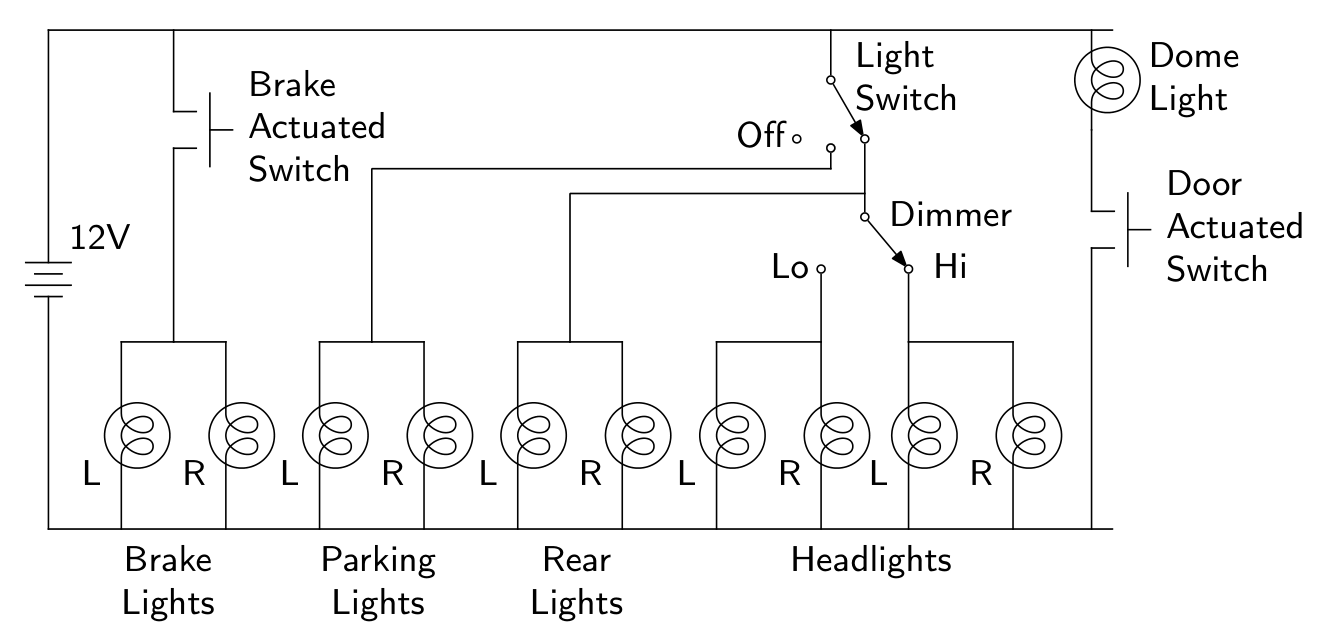
\includegraphics[width=.8\textwidth]{figs/car-circuit}
 \caption{An excerpt from a car's electric network.}
 \label{fig:car-circuit}
\end{figure}

A designer of this network must be able to answer questions similar to: `How
much electricity flows when both the hi-beam headlights and the brake lights are
on?' Even very sophisticated electric networks can be analysed using Kirchhoff's
laws and the theory of linear systems.

The intuitive explanation of electric circuits (which suffices for our purposes)
tells that there are three interconnected forces at play -- voltage $(U)$,
resistance ($R$) and current ($I$). At any point of the circuit, these are tied
by the formula $U = RI$. The battery serves as a capacitor; it provides
\emph{voltage} -- or electric potential -- to the circuit, making electricity
flow as long as there is a path. The moment a path is formed (we say the circuit
is closed), the battery creates a force through the circuit -- the
\emph{current}. Finally, some components of the circuit act as \emph{resistors},
effectively limiting the amount of voltage that is `available' to the subsequent
components of the circuit. This limiting factor is the \emph{resistance} of the
component and is often proportional to the force provided by the battery. We can
think of the resistors causing \emph{voltage drops} throughout the current
whilst the battery provides a \emph{voltage rise}.

To interpret electric networks (basically meshes of electric circuits) as linear
systems, two physical laws are needed -- \emph{Kirchhoff's Current Law} and
\emph{Kirchhoff's Voltage Law}. The former states that at any point in the
network, the flow in equals the flow out. The latter then that around any
circuit in the network, the total voltage rise equals the total voltage drop.

Let us start with a simple network consisting of a single circuit.
\begin{figure}[ht]
 \centering
 \begin{circuitikz}
  \draw (0,0) to [R, l^=$3 \Omega$] (5,0)
        (5,0) to [R, l^=$5 \Omega$] (5,3)
        (5,3) to [R, l^=$2 \Omega$] (0,3)
        (0,3) to [battery, l^=$20 V$] (0,0);
 \end{circuitikz}
 \caption{An electric circuit with a battery and three resistors.}
 \label{fig:electric-network-1}
\end{figure}

The component represented by~\tikz[baseline=.1cm,scale=0.4, every
node/.style={scale=0.4}]{\draw (0,0) to [battery] (0,1);} is the battery
and~\tikz[baseline=-.1cm,scale=0.4, every node/.style={scale=0.4}]{\draw (0,0)
to [R] (1,0);} depicts a resistor. We measure voltage provided by the battery in
\emph{volts} ($V$) and the resistance of the other components in \emph{ohms}
($\Omega$).

Since this network features only a single closed circuit, the current --
measured in \emph{amperes} ($A$) -- is consistent throughout by Kirchhoff's
Current Law. By Kirchhoff's Voltage Law, the total voltage rise (which is $20
V$) equals the total voltage drop. In this circuit, there are three voltage
drops, each equal to the resistance of the component times the current flowing
through it. This gives us a linear system consisting of the single equation
\[
 20 = 2I + 5I + 3I
\]
wherefrom we infer that $I = 2 A$; the current around the circuit equals $2$
amperes.

An example of a network leading to a more elaborate linear system requires
connecting the resistors \emph{in parallel} which automatically creates more
circuits in the network.
\begin{figure}[ht]
 \centering
 \begin{circuitikz}[scale=0.75]
  \draw (0,0) to (7,0)
        (7,0) to (7,1)
        (7,1) to (5,1)
        (5,1) to [R,l^=$12 \Omega$] (5,4)
        (7,1) to (9,1)
        (9,1) to [R,l_=$8 \Omega$] (9,4)
        (5,4) to (7,4)
        (9,4) to (7,4)
        (7,4) to (7,5)
        (7,5) to (0,5)
        (0,5) to [battery,l^=$20 V$] (0,0);
  \draw[-latex,thick] (2,4.7) to node[below] {$i_0$} (5,4.7);
  \draw[-latex,thick] (5.5,3.5) to node[right] {$i_1$} (5.5,1.5);
  \draw[-latex,thick] (8.5,3.5) to node[left] {$i_2$} (8.5,1.5);
 \end{circuitikz}
 \caption{An electric network with resistors connected in parallel.}
 \label{fig:electric-network-2}
\end{figure}

It might not look like it but the network in
\myref{figure}{fig:electric-network-2} actually hosts three circuits depicted in
\myref{figure}{fig:electric-network-3}.
\begin{figure}[ht]
 \centering
 \begin{subfigure}[b]{.3\textwidth}
  \centering
  \begin{circuitikz}[scale=0.3,every node/.style={scale=0.5}]
   \draw[thick,BrickRed]
        (0,0) to (7,0)
        (7,0) to (7,1)
        (7,1) to (5,1)
        (5,1) to [R] (5,4);
   \draw
        (7,1) to (9,1)
        (9,1) to [R] (9,4)
        (9,4) to (7,4);
   \draw[thick,BrickRed]
        (5,4) to (7,4)
        (7,4) to (7,5)
        (7,5) to (0,5)
        (0,5) to [battery] (0,0);
  \end{circuitikz}
  \caption{First \clr{circuit}.}
 \end{subfigure}
 \begin{subfigure}[b]{.3\textwidth}
  \centering
  \begin{circuitikz}[scale=0.3,every node/.style={scale=0.5}]
   \draw[thick,RoyalBlue]
        (0,0) to (7,0)
        (7,0) to (7,1)
        (7,1) to (9,1)
        (7,5) to (0,5)
        (0,5) to [battery] (0,0)
        (9,1) to [R] (9,4)
        (9,4) to (7,4)
        (7,4) to (7,5);
   \draw
        (5,4) to (7,4)
        (7,1) to (5,1)
        (5,1) to [R] (5,4);
  \end{circuitikz}
  \caption{Second \clb{circuit}.}
 \end{subfigure}
 \begin{subfigure}[b]{.3\textwidth}
  \centering
  \begin{circuitikz}[scale=0.3,every node/.style={scale=0.5}]
   \draw[thick,ForestGreen]
        (7,1) to (9,1)
        (9,1) to [R] (9,4)
        (5,1) to [R] (5,4)
        (5,4) to (7,4)
        (9,4) to (7,4)
        (7,1) to (5,1);
   \draw
        (7,4) to (7,5)
        (7,5) to (0,5)
        (0,5) to [battery] (0,0)
        (7,0) to (7,1)
        (0,0) to (7,0);
  \end{circuitikz}
  \caption{Third \clg{circuit}.}
 \end{subfigure}
 \caption{The three circuits of an electric network.}
 \label{fig:electric-network-3}
\end{figure}
Each of those circuits obeys Kirchhoff's Voltage Law. Spelt out for the
\clr{first circuit}, it says the total voltage rise of $20 V$ must equal the
total voltage drop of $12 \Omega$ times the current flowing through this
circuit, which we labelled $i_1$. Similarly, the voltage rise in the \clb{second
circuit} is $20 V$ and equals $8i_2$. Finally, the voltage rise in \clg{circuit
three} is $0 V$ and equals the voltage drop through the first resistor plus the
voltage drop through the second resistor. The only caveat here is the choice of
orientation of the current. The current flowing through the first resistor must
do so in direction opposite to the second resistor as the circuit forms a closed
oriented loop. This means that one of the currents (for instance $i_2$) must be
given a negative sign, signifying a direction of flow opposite to the one in
\clb{circuit two}. This gives a total voltage drop in the \clg{third circuit} as
$12i_1 - 8i_2$.

Finally, there are two points in the network where the flow splits. Applying
Kirchhoff's Current Law thus awards two more equations: $i_0 = i_1 + i_2$ and
$i_1 + i_2 = i_0$. All in all, we ended up with a linear system of five
equations.
\begin{equation}
 \label{eq:electric-network-2}
 \begin{array}{r c r c r c r}
  & & 12i_1 & & & = & 20\\
  & & & & 8i_2 & = & 20\\
  & & 12i_1 & - & 8i_2 & = & 0\\
  i_0 & - & i_1 & - & i_2 & = & 0\\
  -i_0 & + & i_1 & + & i_2 & = & 0
 \end{array}
\end{equation}
Clearly, there are redundant equations in the
system~\eqref{eq:electric-network-2}. This just goes to show that redundancy
arises in practice and the problem of determining which equations are redundant
is generally not entirely trivial; we shall discuss it later in the book.

In this case, of course, the first two equations already give us equalities $i_1
= \frac{5}{3}A$ and $i_2 = \frac{5}{2}A$. Finally, the fourth equation (or the
fifth for that matter) ensures that $i_0 = \frac{25}{6} A$. Hence, the total
current through the entire network is $\frac{25}{6} A$.

The final example to discuss is the so-called
\href{https://en.wikipedia.org/wiki/Wheatstone_bridge}{Wheatstone Bridge}.
\begin{figure}[ht]
 \centering
 \begin{circuitikz}[scale=0.75,every node/.style={scale=0.75}]
  \draw
   (0,0) to (8,0)
   (8,0) to (8,1)
   (8,1) to [R,l^=$10 \Omega$] (5,3)
   (5,3) to [R,l^=$5 \Omega$] (8,5)
   (8,1) to [R,l_=$4 \Omega$] (11,3)
   (11,3) to [R,l_=$2 \Omega$] (8,5)
   (5,3) to [R,l_=$50 \Omega$] (11,3)
   (8,5) to (8,6)
   (8,6) to (0,6)
   (0,6) to [battery,l_=$10 V$] (0,0);
 \end{circuitikz}
 \caption{The \href{https://en.wikipedia.org/wiki/Wheatstone_bridge}{Wheatstone
 Bridge} network.}
 \label{fig:wheatstone-bridge}
\end{figure}
There is \emph{a lot} of circuits in this network. We first choose an arbitrary
orientation of the currents through each of the branches as in
\myref{figure}{fig:wheatstone-bridge-2}.
\begin{figure}[ht]
 \centering
 \begin{circuitikz}[scale=0.5,every node/.style={scale=0.5}]
  \draw
   (0,0) to (8,0)
   (8,0) to (8,1)
   (8,1) to [R] (5,3)
   (5,3) to [R] (8,5)
   (8,1) to [R] (11,3)
   (11,3) to [R] (8,5)
   (5,3) to [R] (11,3)
   (8,5) to (8,6)
   (8,6) to (0,6)
   (0,6) to [battery] (0,0);
  \draw[thick,-latex] (2,5.7) to node[below] {\huge $i_0$} (6,5.7);
  \draw[thick,-latex,shorten <=5pt,shorten >=5pt] (7.7,5.3) to node[above left]
  {\huge $i_1$} (4.7,3.3);
  \draw[thick,-latex,shorten <=5pt,shorten >=5pt] (8.3,5.3) to node[above right]
  {\huge $i_2$} (11.3,3.3);
  \draw[thick,-latex,shorten <=5pt,shorten >=5pt] (4.7,2.7) to node[below left]
  {\huge $i_3$} (7.7,0.7);
  \draw[thick,-latex,shorten <=5pt,shorten >=5pt] (11.3,2.7) to node[below
  right] {\huge $i_4$} (8.3,0.7);
  \draw[thick,-latex,shorten <=8mm,shorten >=8mm,yshift=5mm] (5,3) to
  node[above] {\huge $i_5$} (11,3);
  \draw[thick,-latex] (6,0.3) to node[above] {\huge $i_0$} (2,0.3);
 \end{circuitikz}
 \caption{A choice of current orientation in the
 \href{https://en.wikipedia.org/wiki/Wheatstone_bridge}{Wheatstone Bridge}
network.}
 \label{fig:wheatstone-bridge-2}
\end{figure}

We can't yet be sure how many or which equations we will need to calculate $i_0$
-- the total current. We definitely need at least 6 given the number of
variables. Kirchhoff's Current Law yields many equations but we (based mostly on
intuition) pick these three:
\[
 \begin{array}{r c r c r}
  i_0 & = & i_1 & + & i_2\\
  i_3 & + & i_4 & = & i_0\\
  i_2 & + & i_5 & = & i_4
 \end{array}
\]
We've chosen these particular equations in a way that makes every variable
appear at least once. Using Kirchhoff's Voltage Law on the inner, outer and the
upper `triangle-shaped' circuit gives respectively:
\[
 \begin{array}{r c r c r c r}
  10 & = & 5i_1 & + & 10i_3 & & \\
  10 & = & 2i_2 & + & 4i_4 & & \\
  0 & = & 5i_1 & + & 50i_5 & - & 2i_2
 \end{array}
\]
Again, we have chosen these equations in order to make the resistance of every
component appear at least once. Having collected the six equations into a linear
system, we pray that we get a unique solution.
\[
 \begin{array}{r c r c r c r c r c r c r}
  i_0 & - & i_1 & - & i_2 & & & & & & & = & 0\\
  -i_0 & & & & & + & i_3 & + & i_4 & & & = & 0\\
       & & & & i_2 & & & - & i_4 & + & i_5 & = & 0\\
       & & 5i_1 & & & + & 10i_3 & & & & & = & 10\\
       & & & & 2i_2 & & & + & 4i_4 & & & = & 10\\
       & & 5i_1 & - & 2i_2 & & & & & + & 50i_5 & = & 0
 \end{array}
\]
And\dots~yes! We do. As SageMath confirms.
\begin{Verbatim}
sage: A = \clb{Matrix}(QQ, [
....:     [\clr{1}, \clr{-1}, \clr{-1}, \clr{0}, \clr{0}, \clr{0}],
....:     [\clr{-1}, \clr{0}, \clr{0}, \clr{1}, \clr{1}, \clr{0}],
....:     [\clr{0}, \clr{0}, \clr{1}, \clr{0}, \clr{-1}, \clr{1}],
....:     [\clr{0}, \clr{5}, \clr{0}, \clr{10}, \clr{0}, \clr{0}],
....:     [\clr{0}, \clr{0}, \clr{2}, \clr{0}, \clr{4}, \clr{0}],
....:     [\clr{0}, \clr{5}, \clr{-2}, \clr{0}, \clr{0}, \clr{50}],
....: ])
sage: b = \clb{vector}(QQ, [\clr{0}, \clr{0}, \clr{0}, \clr{10}, \clr{10}, \clr{0}])
sage: A.\clm{solve_right}(b)
(\clr{7/3}, \clr{2/3}, \clr{5/3}, \clr{2/3}, \clr{5/3}, \clr{0})
\end{Verbatim}
A somewhat surprising fact about this solution is the equality $i_5 = 0$,
meaning no electricity flows through the corresponding component.

\begin{exercise}{}{electric-network}
 \myref{Figure}{fig:electric-network-4} depicts an electric network.
 \begin{figure}[H]
  \centering
  \begin{circuitikz}
   \draw
    (0,0) to (3,0)
    (3,0) to [R,l^=$2 \Omega$] (6,0)
    (3,0) to [R,l_=$3 \Omega$] (3,2)
    (6,0) to [R,l^=$2 \Omega$] (9,0)
    (6,0) to [R,l^=$2 \Omega$] (6,2)
    (9,0) to [R,l^=$4 \Omega$] (9,2)
    (3,2) to [R,l_=$3 \Omega$] (6,2)
    (6,2) to [R,l_=$3 \Omega$] (9,2)
    (0,2) to (3,2)
    (0,0) to [battery,l_=$9 V$] (0,2);
  \end{circuitikz}
  \caption{An electric network with 7 resistors.}
  \label{fig:electric-network-4}
 \end{figure}
 Calculate the current in each branch of the network.
\end{exercise}


